% Sandia National Laboratories is a multimission laboratory managed and
% operated by National Technology & Engineering Solutions of Sandia, LLC, a
% wholly owned subsidiary of Honeywell International Inc., for the U.S.
% Department of Energy’s National Nuclear Security Administration under
% contract DE-NA0003525.

% Copyright 2002-2020 National Technology & Engineering Solutions of Sandia,
% LLC (NTESS).

%%-------------------------------------------------------------------------
%% Purpose        : Main LaTeX Xyce Users' Guide
%% Special Notes  : Graphic files (pdf format) work with pdflatex.  To use
%%                  LaTeX, we need to use postcript versions.  Not sure why.
%% Creator        : Scott A. Hutchinson, Computational Sciences, SNL
%% Creation Date  : {05/23/2002}
%%
%%-------------------------------------------------------------------------

% -------------------------------------------------------------------------
% Homotopy/Continuation Analysis Chapter ----------------------------------
% -------------------------------------------------------------------------

\chapter{Homotopy and Continuation Methods}
\label{Homotopy_Chap}
\index{homotopy}

\index{continuation}
\index{continuation}
%\index{bifurcation}

\chapteroverview{Chapter Overview}
{
This chapter includes the following sections:
\begin{XyceItemize}
\item Section~\ref{continuation_Overview}, {\em Continuation Algorithms Overview}
\item Section~\ref{continuation_natural},  {\em Natural Parameter Continuation}
\item Section~\ref{continuation_natural_multiparam}, {\em Natural Multiparameter Continuation}

\item Section~\ref{continuation_gmin},    {\em GMIN Stepping Continuation}
\item Section~\ref{continuation_source},    {\em Source Stepping Continuation}
\item Section~\ref{continuation_mosfet},   {\em MOSFET Continuation}

\item Section~\ref{continuation_pseudotran}, {\em Pseudo Transient}
\item Section~\ref{continuation_arclength}, {\em Arc Length Continuation}
\end{XyceItemize}
}

%%%%%%%%%%%%%%%%%%%%%%%%%%%%%%%%%%%%%%%%%%%%%%%%%%%%%%%%%%%%%%%%%%%%%%%%%%%%%%%%
\section{Continuation Algorithms Overview}

\label{continuation_Overview}
\index{continuation}

Often, circuit convergence problems are most prominent during the DC operating
point calculation. Unlike transient solves, DC operating point analysis cannot
rely on a good initial guess from a previous step, and cannot simply reduce the
step size when the solver fails. Additionally, operating points often have
multiple solutions, with no capability to interpret the user's intent. Multiple
solutions can, even for converged circuit problems, result in a standard Newton
solve being unreliable. For example, the operating point solution to a Schmidt
trigger circuit has been observed to change with the computational platform.

Continuation methods can often provide solutions to difficult nonlinear problems,
including circuit analysis, even when conventional methods (e.g., Newton's
method) fail ~\cite{Melville:1990} ~\cite{Melville:1993}.  This chapter gives
an introduction to using continuation algorithms (sometimes called homotopy 
algorithms) in \Xyce{}. The \Xyce{} Reference Guide\ReferenceGuide{} provides a
more complete description of solver options.

The underlying numerical library used by \Xyce{} to support continuation methods
is LOCA (Library of Continuation Algorithms)~\cite{loca,loca2}.  For a description 
of the numerical details see the LOCA theory and implementation 
manual~\cite{locaManual}.

\subsection{Continuation Algorithms Available in \Xyce{}}

\Xyce{} invokes a well-known SPICE method, ``GMIN stepping,'' automatically
when a DC operating point fails to converge without it.  It is a special case
where the parameter being swept is artificial.  GMIN stepping can also be
invoked with \texttt{.options nonlin continuation=3} or \texttt{.options nonlin
continuation=gmin}. See Section~\ref{continuation_gmin} for more information and an
example of GMIN stepping.

\Xyce{} also invokes the SPICE ``source stepping'' method automatically when a DC operating point calculation fails both normal Newton's method and the automatic GMIN stepping attempt.  This is an example of natural parameter continuation that steps through a scale factor that is applied to all DC voltage sources in the circuit.  It is described in Section~\ref{continuation_source}.

Another basic type of continuation in \Xyce{} is accessed by setting
\texttt{.options nonlin continuation=1}. This allows the user to sweep existing
device parameters (models and instances), as well as a few reserved artificial
parameter cases. The most obvious natural parameter to use is the magnitude(s)
of independent voltage or current sources, the choice of which is equivalent to
``source stepping'' in SPICE.  Section~\ref{continuation_natural} provides a
\Xyce{} source-stepping example.  For some circuits (as in the aforementioned
Schmidt trigger), source stepping leads to turning points in the continuation.  

A special type of continuation, an algorithm designed specifically for MOSFET
circuits~\cite{ROYCHOWDHURY:2003}, involves two internal MOSFET model
parameters---one for the MOSFET gain, and the other for the nonlinearity of the
current-voltage relationship.  This algorithm is invoked with \texttt{.options
nonlin continuation=2}, and has proven to be effective in some large MOSFET
circuits.  Section~\ref{continuation_mosfet} provides a detailed example.

%%%%%%%%%%%%%%%%%%%%%%%%%%%%%%%%%%%%%%%%%%%%%%%%%%%%%%%%%%%%%%%%%%%%%%%%%%%%%%%%
\newpage 
\section{Natural Parameter Continuation}
\label{continuation_natural}
\index{continuation!natural}
\index{continuation!natural}

Figure~\ref{Continuation_Netlist_sourceStepping} shows a natural parameter
continuation netlist with parameters pertinent to the continuation algorithm
highlighted in red.  For this example, the parameter being swept is
the DC value of the voltage source \texttt{VDDdev}.  This
example demonstrates a version of ``source stepping'' that is similar to SPICE,
but only applied to the single voltage source \texttt{VDDdev} rather than to all 
voltage sources.  For an example of source stepping in which every source 
in simultaneously swept, see sections~\ref{continuation_scaling} and~\ref{continuation_source}.

Using continuation on the magnitudes of independent voltage and current sources 
is a fairly obvious technique when a DC operating point calculation fails to 
converge.  However, a na\"{\i}ve application of natural parameter continuation
to single voltage and current sources does not often enable convergence in practice.  
Xyce will apply source stepping automatically during the DC operating point calculation 
if both the standard Newton's method and GMIN stepping fail.  So, normally, this 
technique of manually forcing stepping of a single source is unnecessary.

\begin{figure}[htbp]
\begin{centering}
\shadowbox{
\begin{minipage}{0.8\textwidth}
\begin{vquote}
\color{blue}MOS level 1 model CMOS inverter\color{black}
.TRAN 20ns 30us 0 5ns
.PRINT tran v(vout) v(in) v(1)
.options timeint reltol=5e-3 abstol=1e-3 \color{XyceRed}
* Continuation Options

.options nonlin continuation=1
.options loca stepper=0 predictor=0 stepcontrol=1
+ conparam=VDDdev
+ initialvalue=0.0 minvalue=-1.0 maxvalue=5.0
+ initialstepsize=0.2 minstepsize=1.0e-4 
+ maxstepsize=5.0 aggressiveness=1.0
+ maxsteps=100 maxnliters=200
\color{black}
VDDdev 	VDD	0	5V
RIN	IN	1	1K
VIN1  1	0  5V PULSE (5V 0V 1.5us 5ns 5ns 1.5us 3us)
R1    VOUT  0  10K  
C2    VOUT  0  0.1p 
MN1   VOUT  IN 0   0   CD4012_NMOS  L=5u W=175u         
MP1   VOUT  IN VDD VDD CD4012_PMOS  L=5u W=270u         
.MODEL cd4012_pmos PMOS 
.MODEL cd4012_nmos NMOS 
.END
\end{vquote}
\end{minipage}
}
\caption[Example natural parameter continuation netlist]{Example natural parameter continuation netlist. This example of source stepping shows a circuit that does not require continuation to run. Most circuits complex enough to require continuation would not fit on a single page.\label{Continuation_Netlist_sourceStepping}}
\end{centering}
\end{figure}

\subsection{Explanation of Parameters, Best Practice}
\label{locaParameterExplanation}

Figure~\ref{Continuation_Netlist_sourceStepping} also illustrates the following ``best practice'' rules:

\begin{XyceItemize}
\item \texttt{.options nonlin continuation=1}.  Sets the algorithm to use natural
parameter continuation.
\item \texttt{.options loca conparam=VDDdev}.  If using natural parameter continuation, it is necessary include a setting for \texttt{conparam}.  It sets which input parameter to use to perform continuation.  The parameter name is subject to the same rules as parameter used by the \texttt{.STEP} capability. (Section~\ref{step_InstanceParam}).  In this case, the parameter is the
magnitude of the DC voltage source, VDDdev.  For this type of voltage
source, it was possible to use the default device parameter (Section~\ref{step_SpecialCases})
\item \texttt{.options loca initialvalue=0.0}.  This is required.
\item \texttt{.options loca maxvalue=5.0}.  This is required.
\item \texttt{.options loca stepcontrol=1} or \texttt{.options loca stepcontrol=adaptive}.  This specifies the continuation steps to be adaptive, rather than constant.  This is recommended.
\item \texttt{.options loca maxsteps=100}.  This sets the maximum number of continuation 
steps for each parameter.  
\item \texttt{.options loca maxnliters=200}.  This is the maximum number of nonlinear 
iterations, and has precedence over the similar number that can be set on
the \texttt{.options nonlin} line.
\item \texttt{.options loca aggressiveness=1.0}.  This refers to the step size 
control algorithm,
and the value of this parameter can be anything from 0.0 to 1.0.  1.0 is
the most aggressive.  In practice, try starting with this set to 1.0. 
If the solver fails, then reset to a smaller number.
\end{XyceItemize}

\subsection{Voltage Source Scaling Continuation}
\label{continuation_scaling}
\index{continuation!natural!Voltage Source Scaling}
\index{continuation!natural!Voltage Source Scalaing}

Figure~\ref{Continuation_Netlist_sourceStepping2} shows a natural
parameter continuation netlist with parameters pertinent to the
continuation algorithm highlighted in red.  For this example, a
special parameter \texttt{VSRCSCALE} is being swept from zero to one.
This parameter is applied as a scaling factor for all DC voltage
sources in the netlist.  As a result, this example demonstrates an
explicit invocation of ``source stepping'' like the one that both
\Xyce{} and SPICE apply automatically as part of their DC operating
point solution strategies if Newton's method and GMIN stepping both
fail.

\begin{figure}[htbp]
\begin{centering}
\shadowbox{
\begin{minipage}{0.8\textwidth}
\begin{vquote}
\color{blue}*Simple netlist demonstrating source-stepping continuation
*This source will be swept with .DC \color{black}
V1 1 0 DC 1
R1 1 0 100
\color{blue}*This source will be not swept with .DC \color{black}
V2 2 0 DC 8
R2 2 0 100
.DC V1 1 8 1
.print DC V(1) V(2)
.print HOMOTOPY V(1) V(2)
* Continuation Options
.options nonlin continuation=1

.options loca stepper=0 predictor=0 stepcontrol=0
+ conparam=vsrcscale
+ initialvalue=0.0 minvalue=-1.0 maxvalue=1.0
+ initialstepsize=0.2 minstepsize=1.0e-4 maxstepsize=0.2
+ aggressiveness=1.0
+ maxsteps=5000 maxnliters=200
\color{black}
.END
\end{vquote}
\end{minipage}
}
\caption[Example natural parameter continuation netlist]{Example natural parameter continuation netlist implementing source stepping over all DC voltage sources. This example of source stepping shows a circuit that does not require continuation to run. Most circuits complex enough to require source stepping would not fit on a single page.\label{Continuation_Netlist_sourceStepping2}}
\end{centering}
\end{figure}

%%%%%%%%%%%%%%%%%%%%%%%%%%%%%%%%%%%%%%%%%%%%%%%%%%%%%%%%%%%%%%%%%%%%%%%%%%%%%%%%
\newpage 
\section{Natural Multiparameter Continuation} 
%Per The Chicago Manual of Style, 7.85, ``Compunds formed with prefixes are normally closed, whether %they are nouns, verbs, adjectives, or adverbs.'' There are exceptions, but multiparameter is not one. TT
\label{continuation_natural_multiparam}

It is possible to use the natural parameter continuation specification to  
have \Xyce{} sweep multiple parameters in sequential order.  This 
requires specifying many of the parameters in the \texttt{.options loca} statement as vectors, delineated by commas, rather than as single parameters.  

%An example, which manually reproduces the MOSFET
%continuation example from figure~\ref{Continuation_Netlist_1}, is given in 
%figure~\ref{Continuation_Netlist_multiParam}.

This is a usage example --- the circuit itself does not require continuation to run. Most circuits complex enough to require continuation would not fit on a single page.  

\subsection{Explanation of Parameters, Best Practice}

The solver parameters set in figure~\ref{Continuation_Netlist_multiParam} are 
the same as those from figure~\ref{Continuation_Netlist_sourceStepping}, but many of them
are in vector form.  Specify any parameters specific to the 
continuation variable as a vector, including \texttt{conparam}, \texttt{initialvalue},
 \texttt{minvalue}, \texttt{maxvalue}, \texttt{initialstepsize},
 \texttt{minstepsize}, \texttt{maxstepsize}, and \texttt{aggressiveness}.
Otherwise, the specification is identical.

\begin{figure}[htbp]
\begin{centering}
\shadowbox{
\begin{minipage}{0.8\textwidth}
\begin{vquote}
\color{blue}MOS level 1 model CMOS inverter\color{black}
.TRAN 20ns 30us 0 5ns
.PRINT tran v(vout) v(in) v(1)
.options timeint reltol=5e-3 abstol=1e-3 \color{XyceRed}
* Continuation Options
.options nonlin continuation=1
.options loca stepper=0 predictor=0 stepcontrol=adaptive
+ conparam=mosfet:gainscale,mosfet:nltermscale
+ initialvalue=0.0,0.0 
+ minvalue=-1.0,-1.0 
+ maxvalue=1.0,1.0
+ initialstepsize=0.2,0.2 
+ minstepsize=1.0e-4,1.0e-4 
+ maxstepsize=5.0,5.0 
+ aggressiveness=1.0,1.0
\color{black}
VDDdev 	VDD	0	5V
RIN	IN	1	1K
VIN1  1	0  5V PULSE (5V 0V 1.5us 5ns 5ns 1.5us 3us)
R1    VOUT  0  10K  
C2    VOUT  0  0.1p 
MN1   VOUT  IN 0   0   CD4012_NMOS  L=5u W=175u         
MP1   VOUT  IN VDD VDD CD4012_PMOS  L=5u W=270u         
.MODEL cd4012_pmos PMOS 
.MODEL cd4012_nmos NMOS 
.END
\end{vquote}
\end{minipage}
}
\caption [Example multiparameter continuation netlist]{Example multiparameter continuation netlist. 
This netlist reproduces MOSFET continuation with a manual specification. \label{Continuation_Netlist_multiParam}}


\end{centering}
\end{figure}



%%%%%%%%%%%%%%%%%%%%%%%%%%%%%%%%%%%%%%%%%%%%%%%%%%%%%%%%%%%%%%%%%%%%%%%%%%%%%%%%
\newpage 
\section{GMIN Stepping}
\label{continuation_gmin}
\index{continuation!GMIN Stepping}

GMIN stepping is a type of continuation commonly available in circuit simulators.
Like SPICE, \Xyce{} automatically attempts GMIN stepping if the initial
operating point fails, and if the attempt at GMIN stepping fails, it will subsequently attempt source stepping~\ref{continuation_source}.  As such, it is not typically necessary to manually 
specify GMIN stepping in a \Xyce{} netlist.

However, GMIN stepping may be manually specified by setting
\texttt{continuation=3} or more conveniently, \texttt{continuation=gmin}. If it 
is manually specified, \Xyce{} will \emph{not} attempt to find a DC operating 
point using any other method; it will attempt GMIN stepping, and if that fails 
it will exit with error, not attempting any other method.  Figure~\ref{Gmin_netlist} 
provides a netlist example of GMIN stepping, in which the method has been
explicitly requested.

\begin{figure}[htbp]
\begin{centering}
\shadowbox{
\begin{minipage}{0.8\textwidth}
\begin{vquote}
\color{blue}Simple GMIN stepping example.\color{black}
.TRAN 20ns 30us 0 5ns
.PRINT tran v(vout) v(in) v(1)
.options timeint reltol=5e-3 abstol=1e-3
\color{XyceRed}
* Continuation Options
.options nonlin continuation=gmin 

\color{black}
VDDdev 	VDD	0	5V
RIN	IN	1	1K
VIN1  1	0  5V PULSE (5V 0V 1.5us 5ns 5ns 1.5us 3us)
R1    VOUT  0  10K  
C2    VOUT  0  0.1p 
MN1   VOUT  IN 0   0   CD4012_NMOS  L=5u W=175u         
MP1   VOUT  IN VDD VDD CD4012_PMOS  L=5u W=270u         
.MODEL cd4012_pmos PMOS 
.MODEL cd4012_nmos NMOS 
.END
\end{vquote}
\end{minipage}
}
\caption [Example GMIN stepping netlist.]{Example GMIN stepping netlist. The continuation parameter is gmin. 
It can also be specified using continuation=3. \label  {Gmin_netlist}}
\end{centering}
\end{figure}

The name ''GMIN stepping'' can be somewhat confusing, as ''GMIN'' is
also a user-specified device package parameter (unrelated to this
algorithm) that one may set.  In the device context, ``GMIN'' refers to
a minimum conductance applied to many device models to enhance
convergence.  In the continuation context, it refers to the conductance of
resistors attached from every circuit node to ground.

The conductance, which is the continuation parameter, is initially
very large, and is iteratively reduced until the artificial resistors
have a very high resistance. At the end of the continuation, the
resistors are removed from the problem. At this point, assuming the
continuation has been successful, the original user-specified problem
has been solved.

%%%%%%%%%%%%%%%%%%%%%%%%%%%%%%%%%%%%%%%%%%%%%%%%%%%%%%%%%%%%%%%%%%%%%%%%%%%%%%%%
\newpage 
\section{Source Stepping}
\label{continuation_source}
\index{continuation!Source Stepping}

Source stepping is a type of continuation commonly available in circuit simulators.
Like SPICE, \Xyce{} automatically attempts source stepping if the initial
operating point fails, and if the subsequent attempt at GMIN stepping~\ref{continuation_gmin} 
also fails.  As such, it is not typically necessary to manually 
specify source stepping in a \Xyce{} netlist.

However, source stepping may be manually specified by setting
\texttt{continuation=34} or more conveniently, \texttt{continuation=sourcestep}. If it 
is manually specified,\Xyce{} will \emph{not} attempt to find a DC operating 
point using any other method; it will attempt source stepping, and if that fails 
it will exit with error, not attempting any other method. 
Figure~\ref{sourceStep_netlist} provides a netlist example of source stepping.

\begin{figure}[htbp]
\begin{centering}
\shadowbox{
\begin{minipage}{0.8\textwidth}
\begin{vquote}
\color{blue}Simple test of explicit source stepping
*****************************************\color{black}
R1 1 0 1K 
V1 1 0 5V

.OP
.PRINT DC V(1) I(V1)
.PRINT HOMOTOPY V(1) I(V1)
\color{XyceRed}* Continuation Options
.options nonlin continuation=sourcestep \color{black}

.END\end{vquote}
\end{minipage}
}
\caption [Example source stepping netlist.]{Example source stepping netlist. 
\label  {sourceStep_netlist}}
\end{centering}
\end{figure}

%%%%%%%%%%%%%%%%%%%%%%%%%%%%%%%%%%%%%%%%%%%%%%%%%%%%%%%%%%%%%%%%%%%%%%%%%%%%%%%%
\newpage 
\section{MOSFET Continuation}
\label{continuation_mosfet}
\index{continuation!MOSFET}
\index{continuation!MOSFET}

Figure~\ref{Continuation_Netlist_mos} contains a MOSFET continuation example netlist, and is the same circuit as was used in figure~\ref{Continuation_Netlist_mos}, except some of the parameters are different.  As before, the lines pertinent to the continuation algorithm are highlighted in red.  

\begin{figure}[htbp]
\begin{centering}
\shadowbox{
\begin{minipage}{0.8\textwidth}
\begin{vquote}
THIS CIRCUIT IS A MOS LEVEL 1 MODEL CMOS INVERTER
.TRAN 20ns 30us 0 5ns
.PRINT tran v(vout) v(in) v(1)
.options timeint reltol=5e-3 abstol=1e-3

\color{XyceRed}
* Continuation Options
.options nonlin continuation=mos
\color{black}

VDDdev 	VDD	0	5V
RIN	IN	1	1K
VIN1  1	0  5V PULSE (5V 0V 1.5us 5ns 5ns 1.5us 3us)
R1    VOUT  0  10K  
C2    VOUT  0  0.1p 
MN1   VOUT  IN 0   0   CD4012_NMOS  L=5u W=175u         
MP1   VOUT  IN VDD VDD CD4012_PMOS  L=5u W=270u         
.MODEL cd4012_pmos PMOS 
.MODEL cd4012_nmos NMOS 
.END
\end{vquote}
\end{minipage}
}
\caption[MOSFET continuation netlist example.]{MOSFET continuation netlist example. 
This is a usage example --- the circuit itself does not require continuation to run. Most circuits complex enough to require continuation would not fit on a single page.  
\label{Continuation_Netlist_mos}}
\end{centering}
\end{figure}

\subsection{Explanation of Parameters, Best Practice}

There are a few differences between the netlist in figures~\ref{Continuation_Netlist_sourceStepping} and ~\ref{Continuation_Netlist_mos}. This example shows one set of options, but there are numerous options of working combinations.  

MOSFET continuation requires only \texttt{.options nonlin continuation=2}
or \texttt{.options nonlin continuation=mos} parameters, which
specifies use of the special MOSFET continuation.  This is a two-pass
continuation, in which first a parameter concerning gain is swept from 0
to 1, and then a parameter relating to the nonlinearity of the
transfer curve is swept from 0 to 1.  The default parameters will work
for a variety of MOSFET circuits, so it often will be unneccessary to
override them using an \texttt{.options loca} line. However, it is
possible to override the default parameters using the same
\texttt{.options loca} parameters described in Section
~\ref{locaParameterExplanation}.


%%%%%%%%%%%%%%%%%%%%%%%%%%%%%%%%%%%%%%%%%%%%%%%%%%%%%%%%%%%%%%%%%%%%%%%%%%%%%%%%
\newpage 
\section{Pseudo Transient}
\label{continuation_pseudotran}
\index{continuation!Pseudo Transient}
\index{continuation!Pseudo Transient}

Pseudo transient continuation is very similar to GMIN stepping, in
that both algorithms involve placing large artificial terms on the
Jacobian matrix diagonal, and progressively making these terms smaller
until the original circuit problem is recovered.  One difference is,
rather than doing a series on Newton solves, pseudo transient does a
single nonlinear solve while progressively modifying the pseudo
transient parameter. Figure~\ref{pseudo_netlist_frag} provides an
example of pseudo transient continuation options.

\begin{figure}[htbp]
\begin{centering}
\shadowbox{
\begin{minipage}{0.8\textwidth}
\begin{vquote}

* Continuation Options
.options nonlin continuation=9

.options loca 
+ stepper=natural 
+ predictor=constant 
+ stepcontrol=adaptive
+ initialvalue=0.0
+ minvalue=0.0 
+ maxvalue=1.0e12
+ initialstepsize=1.0e-6 
+ minstepsize=1.0e-6
+ maxstepsize=1.0e6
+ aggressiveness=0.1 
+ maxsteps=200
+ maxnliters=200
+ voltagescalefactor=1.0

\end{vquote}
\end{minipage}
}
\caption [Pseudo transient solver options example.]{Pseudo transient solver options example. The continuation parameter is set to 9. \label{pseudo_netlist_frag}} 
\end{centering}
\end{figure}

\subsection{Explanation of Parameters, Best Practice}

Pseudo transient has not been observed to be as successful as
MOSFET-continuation for large MOSFET circuits. However, it may be a good
candidate for difficult non-MOSFET circuits as it tends to be faster
because the total number of matrix solves is smaller.

%%%%%%%%%%%%%%%%%%%%%%%%%%%%%%%%%%%%%%%%%%%%%%%%%%%%%%%%%%%%%%%%%%%%%%%%%%%%%%%%
\newpage 
\section{Arc Length Continuation}
\label{continuation_arclength} 
Most of the forms of continuation described in this chapter are low-order, and thus
cannot be used to track turning points in the solution.  However, the ability to track
turning points is a capability that can be enabled in \Xyce{}.  A simple example netlist,
which is based on a third order polynomial (which thus has multiple DCOP solutions) is
given in figure~\ref{arclength_netlist}.  The solution, which exhibits this turning
point behavior is given in figure~\ref{arclengthResult}.

\begin{figure}[htbp]
\begin{centering}
\shadowbox{
\begin{minipage}{0.8\textwidth}
\begin{vquote}
\color{blue}Test for turning points using arclength continuation
* polynomial coefficients:\color{black}
.param A=3.0
.param B=-2.0
.param C=1.0
.param I=1.0

Vtest 1 0 5.0
Btest 1 0 V={A*(I(Vtest)-I)**3 + B*(I(Vtest)-I) + C}
.DC Vtest 1 1 1

\color{blue}* natural parameter continuation options (via loca)\color{black}
.options nonlin continuation=1 

\color{blue}* stepper sets what order of continuation this is. 
*   stepper=0 or stepper=NAT  is natural continuation
*   stepper=1 or stepper=ARC  is arclength continuation
*
* predictor must be set to secant to see turning points
*   predictor=0  tangent
*   predictor=1  secant
*   predictor=2  random
*   predictor=3  constant \color{black}
\color{XyceRed}.options loca stepper=1 
+ predictor=1 stepcontrol=1 
+ conparam=Vtest
+ initialvalue=0.0 minvalue=0.0 maxvalue=2.0
+ initialstepsize=0.01 minstepsize=1.0e-8 maxstepsize=0.1
+ aggressiveness=0.1\color{black}
.print homotopy I(Vtest) 
\end{vquote}
\end{minipage}
}
\caption [Arclength continuation example.]{Arclength continuation example.  An explanation of some of the important parameters is given in the comments.  \label{arclength_netlist}} 
\end{centering}
\end{figure}


% Arclength example result
\begin{figure}[ht]
  \centering
  \scalebox{0.7}
  {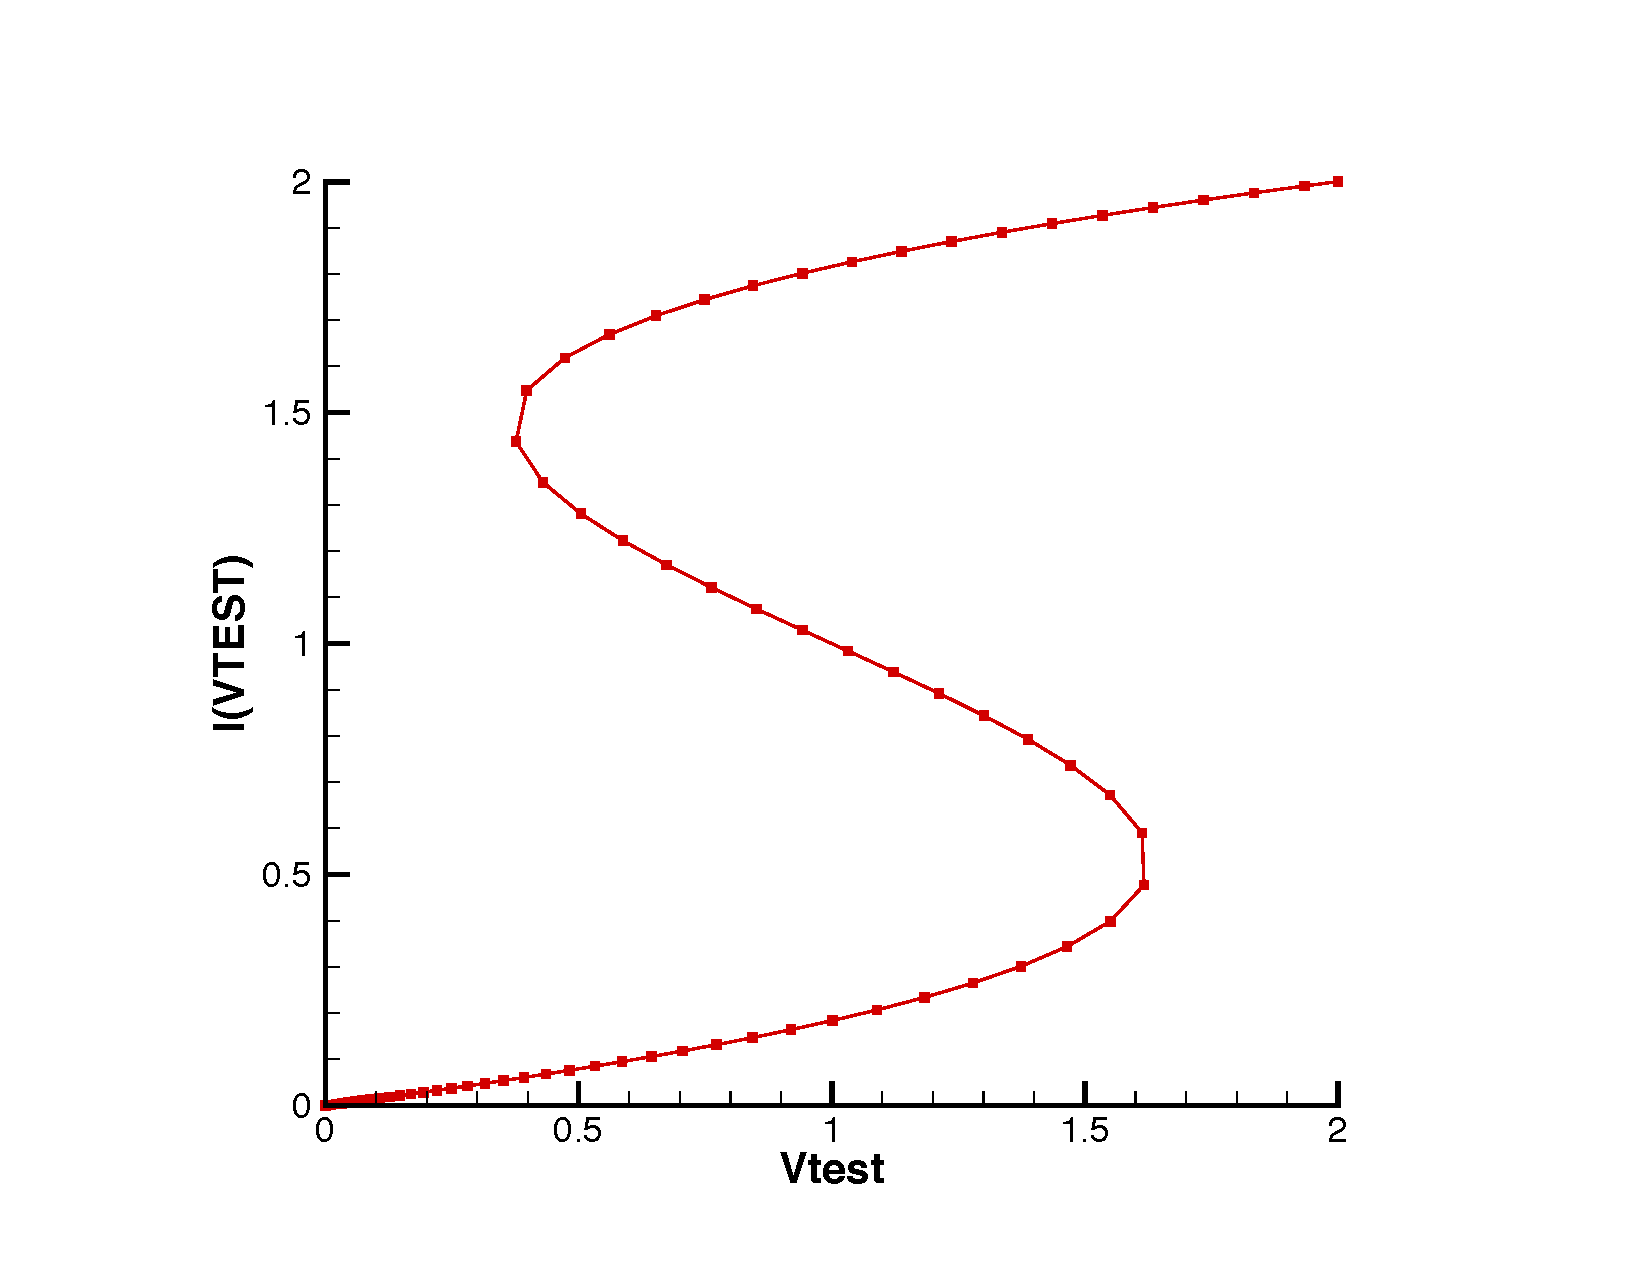
\includegraphics{arclengthSimple}}
  \caption [Arclength continuation example result. ]
  {Arclength continuation example result. This result was generated using \Xyce{} with the netlist in figure~\ref{arclength_netlist}.
\label{arclengthResult}
}
\end{figure}

\subsection{Explanation of Parameters, Best Practice}

Most of the parameters specified in the netlist~\ref{arclength_netlist} are 
the same as the ones described in the natural parameter 
section~\ref{locaParameterExplanation}.  However, two of them must be specified to non-default
values to enable an arclength calculation.   Specifically, the \texttt{stepper} 
parameter must be set to \texttt{1} or \texttt{ARC}, and the \texttt{predictor} 
parameter must be set to \texttt{2} or \texttt{SECANT}. 

%%% Local Variables:
%%% mode: latex
%%% End:

% END of Xyce_UG_ch10.tex ************
